\section{Introduction}

\subsection{Background}
Authentication is the process of confirming the validity of a claimed identity seeking access to a system or resource. Over decades, authentication mechanisms have evolved from basic password systems in the 1960s to advanced methods such as multifactor authentication by the late 2010s, driven by a persistent commitment to combat evolving security risks while enhancing user convenience\cite{ref1}. Various methods such as password-based authentication, certificate-based authentication, one-time passwords, multifactor authentication, and biometric authentication are employed\cite{ref2}.

Biometric authentication, which involves analyzing unique physical characteristics, is often considered more secure than traditional authentication methods due to the difficulty in duplicating biometric traits. This encompasses technologies such as facial recognition, fingerprint recognition, eye recognition, and voice recognition\cite{ref3}.
However, despite the enhanced security of biometric authentication, it is not immune to exploitation. For instance, fingerprints left on surfaces can be copied, or hackers may obtain images of individuals online to deceive authentication systems.
Choosing the right authentication mechanism requires careful consideration of various factors including the necessary security level, ease of use for users, cost implications for setup and ongoing upkeep, as well as the unique risks and vulnerabilities pertinent to the system or data in question. Typically, the requisite level of security steers the selection process; for example, platforms managing sensitive personal information might mandate the use of robust authentication methods, such as biometric verification. The inherent challenge in deploying such secure systems lies in achieving a delicate equilibrium between high security measures and user convenience. The goal is to create an authentication process that is both seamless and efficient, ensuring that access is granted swiftly and accurately to the rightful user without necessitating multiple attempts, thus maintaining a user-friendly experience while upholding the highest security standards.

While advanced biometric systems typically rely on externally visible physical attributes, finger-vein authentication focuses on internal anatomical features, adding a unique layer of security, as they are less prone to replication or theft compared to external characteristics. Nevertheless, it is important to note that finger-vein authentication does not completely eliminate challenges. Despite its emphasis on internal features, attackers can exploit inherent structures in finger veins, such as common patterns among individuals and predictability in acquired data, which poses risks to the authentication process.\\

In light of these considerations, this project is dedicated to authentication using finger-vein features.
This involves utilizing a specialized scanner equipped with two infrared cameras to capture finger veins from different angles.
The registration process involves capturing an image, termed the model image, while the authentication process involves capturing another image, known as the probe image. These images undergo processing through a pipeline designed to extract and align the finger-vein patterns.
The pipeline outputs a feature vector, which is essentially a bitstring, where 0's represent where there are no finger veins, and 1's show where veins are present.
Following this process, the system evaluates whether the feature vector extracted from the probe image sufficiently matches the feature vector of the model image associated with the individual attempting authentication.

\subsection{Extraction Pipeline}\label{sec:extraction-pipeline}

This project extends the work on optimizing a finger-vein recognition pipeline that has demonstrated the lowest \hyperref[def:EER]{Equal Error Rate (EER)} by incorporating a novel hashing step to process the output of the pipeline. The purpose of integrating \hyperref[def:Hash_Function]{Hash Functions} within this context is multifold, but before delving into hash functions, which are central to our project, it's essential to outline the foundation upon which we have built our advancements. This initial context will provide a clearer understanding of the starting point from which our developments began.\\

Simon Sommerhalder and Burcu Yildiz have both made significant contributions to the system. Simon introduced an innovative approach to the alignment of freshly captured images (probe images) with those stored in the system (model images), ensuring the hashing process (following the alignment of the finger) is based on the unique finger-vein pattern rather than how the finger is positioned on the scanner.

Simon has developped a pipeline (see Figure~\ref{pipeline_simon}) to align finger-vein images, enhancing security by eliminating the need to compare the model and probe images side by side. He organized the pipeline into six clear steps:

\begin{enumerate}
    \item \textbf{Masking}: The first step of the pipeline isolates the finger area in the image. This involves creating a mask that outlines the finger, ensuring that subsequent processing focuses solely on the relevant part of the image.

    \item \textbf{Prealignment}: This step involves adjusting the position and orientation of the finger within the image before extracting vein patterns. It's aimed at roughly aligning the image based on the finger's outline, helping to standardize the position of the finger across different scans.

    \item \textbf{Histogram equalization}: To ensure the images have consistent lighting and contrast, this step adjusts the brightness levels. This makes the vein patterns more distinct and comparable across different images.

    \item \textbf{Feature extraction}: Here, the actual vein patterns are identified and extracted from the image. The process converts the visual image into a digital format that represents the presence or absence of veins at specific locations.

    \item \textbf{Postalignment}: After extracting the vein patterns, this step fine-tunes the alignment of the image. It's based on the vein patterns themselves, ensuring that the comparison between model and probe images is as accurate as possible.

    \item \textbf{Distance Calculation}: The final step involves comparing the feature vector of the probe image with that of the model image. This is done using a specific metric to quantify the similarity between the two, ultimately determining if they match closely enough for authentication to succeed.
\end{enumerate} 

\begin{figure}[!h]
    \centering
    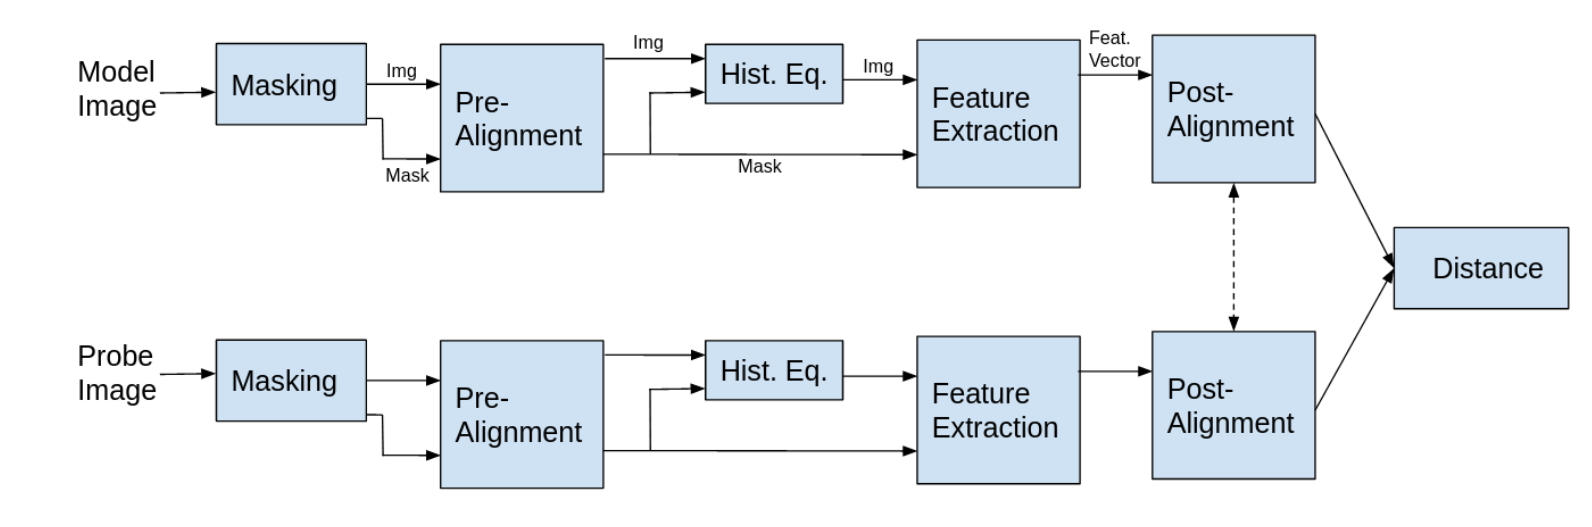
\includegraphics[width=1\linewidth]{latex-img/pipeline_simon.png}
    \caption{Simon's Extraction Pipeline. Compares a single probe image to a model image}
    \label{pipeline_simon}
\end{figure}

Burcu's work on the finger vein authentication project built upon Simon's foundational pipeline, focusing on refining image processing for vein extraction and evaluating different distance calculation methods for authentication. She optimized preprocessing steps, investigated masking and prealignment issues, and tackled reference selection to enhance matching accuracy. A significant part of her contributions involved exploring fuzzy extractors \hyperref[def:Fuzzy_Extractors]{Fuzzy Extractors} to bolster security, conducting a thorough analysis of the dataset to identify and address challenges, and proposing solutions to improve the system's reliability and efficiency.\\

Simon and Burcu explored a variety of function combinations at different stages of the authentication pipeline, aiming to pinpoint the configuration that yields the most favorable outcomes. They utilized the Equal Error Rate (EER) as a benchmark to measure the pipeline's efficacy, focusing on achieving a balance between security and accessibility. This metric, representing the point where the rate of false acceptances (impostor incorrectly granted access) matches the rate of false rejections (legitimate user incorrectly denied), serves as an indicator of the system's reliability and accuracy. The configuration that demonstrated superior performance, leading to the lowest EER and thereby optimizing the process of analyzing and processing images, is showcased in the subsequent figure.

\begin{table}[H]
    \centering
    \caption{EER values for the best pipeline: Edge masking, translation pre-alignment, no pre-processing, no post-
    processing, Miura matching as the post-alignment}
    \begin{tabular}{lc}
    \toprule
    Camera & EER \\
    \midrule
    Camera 1 & 0.041 \\
    Camera 2 & 0.029 \\
    Sum of cameras & 0.030 \\
    \bottomrule
    \end{tabular}
    \label{tab:eervalues_best}
\end{table}

\subsection{Project Overview}

In the progression of our project, building upon the work of Simon and Burcu, we aim to address the inherent variability in biometric data, particularly with finger vein patterns, by considering hash functions. The final objective of the system is to add a hashing step at the end of our established pipeline, prior to the post-alignment phase. The integration of this step serves to enhance security and overall functionality by allowing us to store a hash of each biometric image X in our database, instead of the raw biometric data. Upon receiving a new image Y, we compute hashes for all potential translations of Y, comparing these with the hash of X. Unfortunately, this process is computationally expensive because it requires computing the hash for every possible translation of the image. The purpose of employing a hashing process in this system is multifold:

\begin{itemize}
    \item \textbf{Security}: Hash values can be stored instead of raw biometric data. In the event of a database breach, attackers would find it significantly more challenging to reconstruct the original biometric information from the hashed values due to the one-way nature of hash functions.

    \item \textbf{Consistency}: By focusing on the unique patterns of the biometric trait (like finger-vein patterns) and standardizing how this data is processed and hashed, the system aims to produce consistent hash values for the same individual across different scanning sessions. This is crucial for reliable authentication, ensuring that minor variations in finger placement do not affect the system's ability to recognize the user.

    \item \textbf{Performance}: Hashing biometric data into a compact, fixed-size format facilitates quicker comparison and verification processes. It's more efficient to compare hash values than to perform complex pattern recognition operations on raw biometric images.
\end{itemize}

Traditional hash functions, while pivotal in various data security contexts, generate a unique output for each unique input. This one-to-one mapping means even minor variations in the input — common in biometric data due to natural changes in biological traits or differences in scanning conditions — result in completely different hashes. This sensitivity to input variability poses a challenge in biometric authentication systems, where the goal is to accurately recognize and authenticate an individual despite these natural variations.

Fuzzy hashing stands as a sophisticated solution to this challenge. Unlike traditional hash functions, fuzzy hashing is designed to produce consistent cryptographic keys for inputs that are similar, but not identical. This is particularly advantageous in biometric authentication systems, where it's essential to recognize the same biometric trait across different instances, despite slight variations. The "fuzziness" of this approach allows the system to map these similar inputs to the same or closely related hash values, thereby ensuring that legitimate users are not incorrectly denied access due to minor discrepancies in their biometric data.
Furthermore, the application of fuzzy hashing in our pipeline is instrumental in protecting user privacy. Since the hashed values, rather than raw biometric data, are stored and used for authentication, users' biometric information is safeguarded against potential breaches. Even if hashed values were accessed without authorization, the complexity of fuzzy hashing algorithms makes it extremely challenging to reverse-engineer the original biometric data.\\

The process of our fuzzy hashing algorithm, that we will detail in Section~\ref{sec:Fuzzy Hashing}  begins with a biometric capture, a finger image, which goes through the already developped pipeline~\ref{pipeline_simon} to extract a bitstring. This bitstring undergoes a pre-hashing process, where a subset of significant bits (denoted as vein pixels) is selected based on a permutation keyed by a secure key, resulting in a tuple that significantly reduces the data's dimensionality while preserving its distinguishing features.

Upon generating the fuzzy hash, the next step involves further compressing this hash to prepare it for storage. This compression is achieved through a function, postHash, which maps the tuple to a bitstring of a defined length. The output, essentially a compressed fuzzy hash, exhibits nearly uniform distribution when both the input data and the key are random, enhancing security and storage efficiency.

To further bolster the security of the stored biometric data, this system incorporates \hyperref[def:Fuzzy_Extractors]{Fuzzy Extractors}. The fuzzy extractor framework ensures that even if the stored data is compromised, reconstructing the original biometric data or compromising individual privacy remains computationally infeasible. This is accomplished by generating a secure, random key from the biometric input using a generation process (Gen) and allowing for the reliable reproduction of this key from an approximation of the original input using a reproduction process (Rep), without directly storing the biometric data itself.

In essence, we aim to store the output of the fuzzy extractor, which includes the reproducible cryptographic key and the helper data, instead of the raw biometric data or its direct hash. This method ensures that the stored biometric data is not only compact and efficiently stored but also securely obfuscated, requiring the correct biometric input for any form of decryption or matching to occur.


\section{Introduction}

\subsection{Background}
Authentication is the process of confirming the validity of a claimed identity seeking access to a system or resource. Over decades, authentication mechanisms have evolved from basic password systems in the 1960s to advanced methods such as multifactor authentication by the late 2010s, driven by a persistent commitment to combat evolving security risks while enhancing user convenience\cite{ref1}. Various methods such as password-based authentication, certificate-based authentication, one-time passwords, multifactor authentication, and biometric authentication are employed\cite{ref2}.

Biometric authentication, which involves analyzing unique physical characteristics, is often considered more secure than traditional authentication methods due to the difficulty in duplicating biometric traits. This encompasses technologies such as facial recognition, fingerprint recognition, eye recognition, and voice recognition\cite{ref3}.
However, despite the enhanced security of biometric authentication, it is not immune to exploitation. For instance, fingerprints left on surfaces can be copied, or hackers may obtain images of individuals online to deceive authentication systems.
Choosing the right authentication mechanism requires careful consideration of various factors including the necessary security level, ease of use for users, cost implications for setup and ongoing upkeep, as well as the unique risks and vulnerabilities pertinent to the system or data in question. Typically, the requisite level of security steers the selection process; for example, platforms managing sensitive personal information might mandate the use of robust authentication methods, such as biometric verification. The inherent challenge in deploying such secure systems lies in achieving a delicate equilibrium between high security measures and user convenience. The goal is to create an authentication process that is both seamless and efficient, ensuring that access is granted swiftly and accurately to the rightful user without necessitating multiple attempts, thus maintaining a user-friendly experience while upholding the highest security standards.

While advanced biometric systems typically rely on externally visible physical attributes, finger-vein authentication focuses on internal anatomical features, adding a unique layer of security, as they are less prone to replication or theft compared to external characteristics. Nevertheless, it is important to note that finger-vein authentication does not completely eliminate challenges. Despite its emphasis on internal features, attackers can exploit inherent structures in finger veins, such as common patterns among individuals and predictability in acquired data, which poses risks to the authentication process.\\

In light of these considerations, this project is dedicated to authentication using finger-vein features.
This involves utilizing a specialized scanner equipped with two infrared cameras to capture finger veins from different angles.
The registration process involves capturing an image, termed the model image, while the authentication process involves capturing another image, known as the probe image. These images undergo processing through a pipeline designed to extract and align the finger-vein patterns.
The pipeline outputs a feature vector, which is essentially a bitstring, where 0's represent where there are no finger veins, and 1's show where veins are present.
Following this process, the system evaluates whether the feature vector extracted from the probe image sufficiently matches the feature vector of the model image associated with the individual attempting authentication.

\subsection{Extraction Pipeline}\label{sec:extraction-pipeline}

This project extends the work on optimizing a finger-vein recognition pipeline that has demonstrated the lowest \hyperref[def:EER]{Equal Error Rate (EER)} by incorporating a novel hashing step to process the output of the pipeline. The purpose of integrating \hyperref[def:Hash_Function]{Hash Functions} within this context is multifold, but before delving into hash functions, which are central to our project, it's essential to outline the foundation upon which we have built our advancements. This initial context will provide a clearer understanding of the starting point from which our developments began.\\

Simon Sommerhalder and Burcu Yildiz have both made significant contributions to the system. Simon introduced an innovative approach to the alignment of freshly captured images (probe images) with those stored in the system (model images), ensuring the hashing process (following the alignment of the finger) is based on the unique finger-vein pattern rather than how the finger is positioned on the scanner.

Simon has developped a pipeline (see Figure~\ref{pipeline_simon}) to align finger-vein images, enhancing security by eliminating the need to compare the model and probe images side by side. He organized the pipeline into six clear steps:

\begin{enumerate}
    \item \textbf{Masking}: The first step of the pipeline isolates the finger area in the image. This involves creating a mask that outlines the finger, ensuring that subsequent processing focuses solely on the relevant part of the image.

    \item \textbf{Prealignment}: This step involves adjusting the position and orientation of the finger within the image before extracting vein patterns. It's aimed at roughly aligning the image based on the finger's outline, helping to standardize the position of the finger across different scans.

    \item \textbf{Histogram equalization}: To ensure the images have consistent lighting and contrast, this step adjusts the brightness levels. This makes the vein patterns more distinct and comparable across different images.

    \item \textbf{Feature extraction}: Here, the actual vein patterns are identified and extracted from the image. The process converts the visual image into a digital format that represents the presence or absence of veins at specific locations.

    \item \textbf{Postalignment}: After extracting the vein patterns, this step fine-tunes the alignment of the image. It's based on the vein patterns themselves, ensuring that the comparison between model and probe images is as accurate as possible.

    \item \textbf{Distance Calculation}: The final step involves comparing the feature vector of the probe image with that of the model image. This is done using a specific metric to quantify the similarity between the two, ultimately determining if they match closely enough for authentication to succeed.
\end{enumerate} 

\begin{figure}[!h]
    \centering
    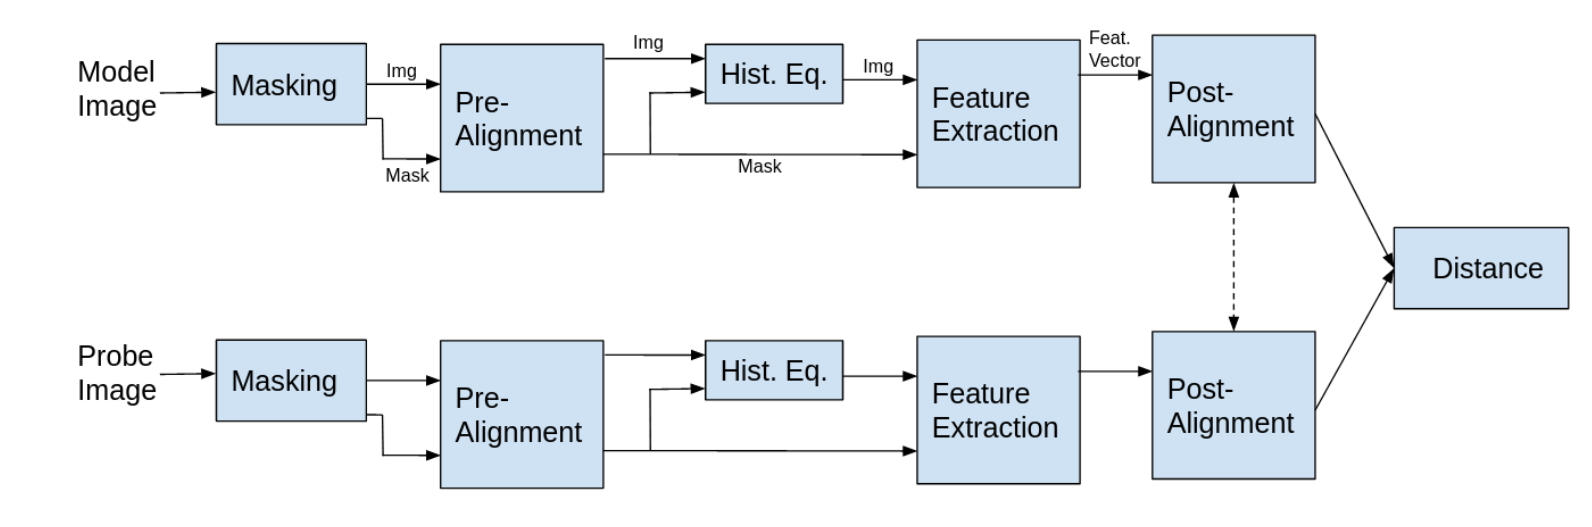
\includegraphics[width=1\linewidth]{latex-img/pipeline_simon.png}
    \caption{Simon's Extraction Pipeline. Compares a single probe image to a model image}
    \label{pipeline_simon}
\end{figure}

Burcu's work on the finger vein authentication project built upon Simon's foundational pipeline, focusing on refining image processing for vein extraction and evaluating different distance calculation methods for authentication. She optimized preprocessing steps, investigated masking and prealignment issues, and tackled reference selection to enhance matching accuracy. A significant part of her contributions involved exploring fuzzy extractors \hyperref[def:Fuzzy_Extractors]{Fuzzy Extractors} to bolster security, conducting a thorough analysis of the dataset to identify and address challenges, and proposing solutions to improve the system's reliability and efficiency.\\

Simon and Burcu explored a variety of function combinations at different stages of the authentication pipeline, aiming to pinpoint the configuration that yields the most favorable outcomes. They utilized the Equal Error Rate (EER) as a benchmark to measure the pipeline's efficacy, focusing on achieving a balance between security and accessibility. This metric, representing the point where the rate of false acceptances (impostor incorrectly granted access) matches the rate of false rejections (legitimate user incorrectly denied), serves as an indicator of the system's reliability and accuracy. The configuration that demonstrated superior performance, leading to the lowest EER and thereby optimizing the process of analyzing and processing images, is showcased in the subsequent figure.

\begin{table}[H]
    \centering
    \caption{EER values for the best pipeline: Edge masking, translation pre-alignment, no pre-processing, no post-
    processing, Miura matching as the post-alignment}
    \begin{tabular}{lc}
    \toprule
    Camera & EER \\
    \midrule
    Camera 1 & 0.041 \\
    Camera 2 & 0.029 \\
    Sum of cameras & 0.030 \\
    \bottomrule
    \end{tabular}
    \label{tab:eervalues_best}
\end{table}

\subsection{Project Overview}

In the progression of our project, building upon the work of Simon and Burcu, we aim to address the inherent variability in biometric data, particularly with finger vein patterns, by considering hash functions. The final objective of the system is to add a hashing step at the end of our established pipeline, prior to the post-alignment phase. The integration of this step serves to enhance security and overall functionality by allowing us to store a hash of each biometric image X in our database, instead of the raw biometric data. Upon receiving a new image Y, we compute hashes for all potential translations of Y, comparing these with the hash of X. Unfortunately, this process is computationally expensive because it requires computing the hash for every possible translation of the image. The purpose of employing a hashing process in this system is multifold:

\begin{itemize}
    \item \textbf{Security}: Hash values can be stored instead of raw biometric data. In the event of a database breach, attackers would find it significantly more challenging to reconstruct the original biometric information from the hashed values due to the one-way nature of hash functions.

    \item \textbf{Consistency}: By focusing on the unique patterns of the biometric trait (like finger-vein patterns) and standardizing how this data is processed and hashed, the system aims to produce consistent hash values for the same individual across different scanning sessions. This is crucial for reliable authentication, ensuring that minor variations in finger placement do not affect the system's ability to recognize the user.

    \item \textbf{Performance}: Hashing biometric data into a compact, fixed-size format facilitates quicker comparison and verification processes. It's more efficient to compare hash values than to perform complex pattern recognition operations on raw biometric images.
\end{itemize}

Traditional hash functions, while pivotal in various data security contexts, generate a unique output for each unique input. This one-to-one mapping means even minor variations in the input — common in biometric data due to natural changes in biological traits or differences in scanning conditions — result in completely different hashes. This sensitivity to input variability poses a challenge in biometric authentication systems, where the goal is to accurately recognize and authenticate an individual despite these natural variations.

Fuzzy hashing stands as a sophisticated solution to this challenge. Unlike traditional hash functions, fuzzy hashing is designed to produce consistent cryptographic keys for inputs that are similar, but not identical. This is particularly advantageous in biometric authentication systems, where it's essential to recognize the same biometric trait across different instances, despite slight variations. The "fuzziness" of this approach allows the system to map these similar inputs to the same or closely related hash values, thereby ensuring that legitimate users are not incorrectly denied access due to minor discrepancies in their biometric data.
Furthermore, the application of fuzzy hashing in our pipeline is instrumental in protecting user privacy. Since the hashed values, rather than raw biometric data, are stored and used for authentication, users' biometric information is safeguarded against potential breaches. Even if hashed values were accessed without authorization, the complexity of fuzzy hashing algorithms makes it extremely challenging to reverse-engineer the original biometric data.\\

The process of our fuzzy hashing algorithm, that we will detail in Section~\ref{sec:Fuzzy Hashing}  begins with a biometric capture, a finger image, which goes through the already developped pipeline~\ref{pipeline_simon} to extract a bitstring. This bitstring undergoes a pre-hashing process, where a subset of significant bits (denoted as vein pixels) is selected based on a permutation keyed by a secure key, resulting in a tuple that significantly reduces the data's dimensionality while preserving its distinguishing features.

Upon generating the fuzzy hash, the next step involves further compressing this hash to prepare it for storage. This compression is achieved through a function, postHash, which maps the tuple to a bitstring of a defined length. The output, essentially a compressed fuzzy hash, exhibits nearly uniform distribution when both the input data and the key are random, enhancing security and storage efficiency.

To further bolster the security of the stored biometric data, this system incorporates \hyperref[def:Fuzzy_Extractors]{Fuzzy Extractors}. The fuzzy extractor framework ensures that even if the stored data is compromised, reconstructing the original biometric data or compromising individual privacy remains computationally infeasible. This is accomplished by generating a secure, random key from the biometric input using a generation process (Gen) and allowing for the reliable reproduction of this key from an approximation of the original input using a reproduction process (Rep), without directly storing the biometric data itself.

In essence, we aim to store the output of the fuzzy extractor, which includes the reproducible cryptographic key and the helper data, instead of the raw biometric data or its direct hash. This method ensures that the stored biometric data is not only compact and efficiently stored but also securely obfuscated, requiring the correct biometric input for any form of decryption or matching to occur.


\section{Biometric Setting}
\label{sec:bio_setting}
This section provides a comprehensive overview of the mathematical and technical aspects involved in fingervein matching, which is essential for comprehending the subsequent discussions in this paper. Additionally, insights into the process of obtaining these equations and statements will be provided, evaluating their relevance and implications within the context of the research. 

\subsection{Biometric Data and Similarity Scores}
\label{Bio_data_sim_scores}
We begin by delving into the representation of the biometric data. Finger images, designated as biometric templates and formated as \(250\)x\(386\), result in \(n\) = \(96'500\) pixels per image. To enhance processing efficiency, these templates are converted into vectors, departing from their original 2-dimension image structure. 

In the biometric context, each finger serves as a biometric subject, with a corresponding biometric capture represented as a bitstring \(X\) of length \(n\). This capture encapsulates the specific vein pixel information extracted from the finger image, while the biometric template serves as a reference mode derived from these images. 

Each of the \(n\) bits of the biometric capture is designated as \(X_1, \ldots, X_n\), with \(X_i\) set to \(1\) if the \(i\)-th bit corresponds to a vein and \(0\) otherwise. We define a random variable as the Hamming Weight of a feature vector \(X\) divided by the total number of bits in the vector \(\left( \frac{\text{HW}(X)}{n} \right)\). The parameter \(p\) is defined as the mean of this random variable.

\begin{equation} \label{eq:p}
    \begin{aligned}
        p = \mathbb{E}\left( \frac{\text{HW}(X)}{n} \right) = Pr\left(X_i = 1\right)
    \end{aligned}
\end{equation}

In the case where \(i\) is a uniformly distributed random index and \(X\) is randomly chosen, the mean (\(p\))\footnote{Throughout this report, experimentally derived variables are denoted with the superscript "obs" (e.g., \(\text{var}^{\text{obs}}\)), while theoretical variables are presented without any superscript.}, along with the variance (\(\sigma²\)) and standard deviation (\(\sigma\)) of the random variable \(\frac{\text{HW}(X)}{n}\) across all images are quantified as follows:

\begin{equation} \label{eq:proba1}
    p^{\text{obs}} = \mathbb{E}\left( \frac{\text{HW}(X)}{n} \right) = 3.29\%
\end{equation}

\begin{equation} \label{eq:proba2}
    \sigma^{\text{obs}} = \sqrt{\mathbb{E} \left[ \left( \frac{\text{HW}(X)}{n} - p^{\text{obs}} \right)^2 \right]} \approx 4.69 \times 10^{-3}
\end{equation}


\begin{equation} \label{eq:proba3}
    (\sigma^{\text{obs}})² = \mathbb{V}\left( \frac{\text{HW}(X)}{n} \right)  \approx 2.20 \times 10^{-5}
\end{equation}

where \( \sigma \) and \( \sigma^2 \) represent the standard deviation and variance of the random variable \(\frac{\text{HW}(X)}{n}\) respectively.

In biometric authentication and identification, the uniqueness of each biometric capture is encoded in its bits. The objective revolves around discerning the similarity between two biometric captures to verify or identify two individuals. Therefore, the scoring mechansim plays a crucial role in quantatively determining the similarity between biometric captures. This similarity score holds significance in verifying the identity of an individual (authentication) or identifying potential matches in a database (identification). A higher score indicates a greater ressemblance between captures, while a lower score suggests less similarity. This scoring mechanism is indispensable for ensuring the accuracy and reliability of biometric systems. The score of (\(X\), \(Y\)) is computed as

\begin{equation} \label{eq:score}
    \begin{aligned}
        Score(X, Y) &= \frac{HW(X \land Y)}{HW(X) + HW(Y)}\\
        &= \frac{1}{2}-\frac{1}{2}\frac{d_H(X, Y)}{HW(X) + HW(Y)}
    \end{aligned}
\end{equation}

where \(HW\) denotes the \hyperref[def:Hamming Weight]{Hamming Weight} and \(d_H\) the \hyperref[def:Hamming Distance]{Hamming Distance}. 

In conjunction with the scoring mechanism, Miura matching emerges as a specialized technique for comparing biometric samples. This method entails determining an optimal offset translation, denoted as \(d_X\) and \(d_Y\), between two biometric samples to align their features for comparison, thereby compensating for differences in positioning or orientation. The alignment process maximizes the similarity score, defined as:

\[Score = \text{Score}(d_X \cdot X, d_Y \cdot Y)\]

Once the optimal offsets, \(d_X\) and \(d_Y\), are determined, they are applied to the original samples for alignment. This results in the calculated aligned positions, denoted as \(\bar{X}\) and \(\bar{Y}\), such that:

\[\bar{X} = d_X \cdot X\]
\[\bar{Y} = d_Y \cdot Y\]

Miura matching and the scoring mechanism are interconnected components, where Miura matching facilitates the computation of the score, thereby offering insights into the similarity between biometric captures and enhancing the reliability of matching algorithms.

The probability of the \(i\)-th pixel of two captures not being the same after applying the optimal offset translations depends on the distribution of \((\bar{X}, \bar{Y})\), and is denoted as \(\delta\). We define the random variable as the normalized Hamming distance between two feature vectors \(\left( \frac{d_H(\bar{X}, \bar{Y})}{n} \right)\). The parameter \(\delta\) is defined as the mean of this random variable, and we additionally define the standard deviation and the variance of this random variable, as shown in the following figures.



\begin{equation} \label{eq:delta}
    \begin{aligned}
        \delta = \mathbb{E}\left( \frac{d_H(\bar{X}, \bar{Y})}{n} \right)
    \end{aligned}
\end{equation}

\begin{equation}
    \begin{aligned}
        \sigma_{\delta} = {\sigma}\left( \frac{d_H(\bar{X}, \bar{Y})}{n} \right)
    \end{aligned}
\end{equation}

\begin{equation}
    \begin{aligned}
        \sigma^2_{\delta} = {Var}\left( \frac{d_H(\bar{X}, \bar{Y})}{n} \right)
    \end{aligned}
\end{equation}

Distinguishing between the types of distributions associated with the two captures is crucial. When both captures originate from the same biometric subject, it is referred to as \(\delta_{\text{same}}\). Conversely, if the captures are from different subjects, it is labeled as \(\delta_{\text{diff}}\). Additionally, when \(\bar{X}\) and \(\bar{Y}\) consist of \(2n\) independent random bits with an expected value of \(p\) and no optimal offset is applied, it is classified as \(\delta_{\text{indep}}\). In this scenario, \(\delta_{\text{indep}}^{\text{obs}} = 2p(1-p) = 6.4\%\). As developed in Section~\ref{sec:delta}, the experimental results produce the following figures:

\begin{table}[H]
    \centering
    \renewcommand{\arraystretch}{1.25}
    \begin{tabular}{|c|c|c|c|}
        \hline
        & \textbf{\(\delta^{\text{obs}}\)} & \textbf{\({\sigma^2_{\delta}}^{\text{obs}}\)} & \textbf{\(\sigma_{\delta}^{\text{obs}}\)} \\
        \hline
        \text{Same-Finger Distribution} & 4.55\% & \(1.06 \times 10^{-4}\) & \(1.03 \times 10^{-2}\) \\
        \hline
        \text{Different-Finger Distribution} & 5.99\% & \(4.58 \times 10^{-5}\) & \(6.76 \times 10^{-3}\) \\
        \hline
    \end{tabular}
    \caption{Comparison of Distributions: Mean, Variance, and Standard Deviation of \(\frac{d_H(\bar{X}, \bar{Y})}{n}\) when both captures originate from the same finger and from different fingers}
\end{table}


Utilizing \(p\) (\ref{eq:p}) and $\delta$ (\ref{eq:delta}), the joint distribution for (\(\bar{X}_j\), \(\bar{Y}_j\)) across \(j\) random instances is derived:

\begin{table}[H]
    \centering
    \renewcommand{\arraystretch}{1.5}
    \begin{tabular}{|c|c|c|}
        \hline
        & $\bar{Y}_i = 0$ & $\bar{Y}_i = 1$\\
        \hline
        $\bar{X}_i = 0$ & $1 - p - \frac{\delta}{2}$ & $\frac{\delta}{2}$\\
        \hline
        $\bar{X}_i = 1$ & $\frac{\delta}{2}$ & $p - \frac{\delta}{2}$\\
        \hline
    \end{tabular}
    \caption{Joint Distribution of ($\bar{X}_j$, $\bar{Y}_j$) for Random Instances}
    \label{tab:joint_distribution}
\end{table}

\subsection{Experimental Derivation of the Probability \(p\)}

In order to derive the probability that a distributed random pixel is a vein, \(p\) (\ref{eq:p}), a dataset of 20 unique individuals was utilized. Each individual contributed images of both right and left index/middle fingers, with 5 trials per finger, captured using 2 different cameras. This methodology resulted in a comprehensive dataset of 800 images. Following the approach in Section~\ref{sec:extraction-pipeline}, Simon's optimal pipeline was implemented to extract the feature vectors from each image in the dataset (refer to Figure~\ref{pipeline_simon}). Subsequently, statistical analysis was performed on these feature vectors to gain insights into vein patterns, building on the preliminary work by Burcu. It's important to note that the calculation of the probability \(p\) does not take into account any postalignment method, like Miura Matching, even though the code might seem like it does.

We have carried out this analysis by implementing an algorithm which processes the dataset's feature vectors, performing two main functions:
\begin{enumerate}
    \item For each pixel position, it updates a \textit{veins[i]} array, which accumulates detections of veins across all images for each camera \(i={1,2}\).
    \item It maintains a count of the number of images analyzed per camera \(i={1,2}\) in a \textit{image\_count[i]} array.
\end{enumerate}

Following the processing of all feature vectors, the algorithm computes the probability of a pixel being part of a vein by dividing the aggregated vein detections by the total number of images analyzed, across both cameras. Visual representations were generated to illustrate the distribution of detected vein pixels for each camera individually and for the combined data from both cameras.
\newpage
\begin{enumerate}
    \item \textbf{Camera 1 and Camera 2 distribution}: The following histograms showcase the frequency distribution of vein pixels detected in images captured by Camera 1 and 2 individually, with a Gaussian fit overlaid to highlight the data's normal distribution trend.

    \begin{figure}[H]
        \centering
        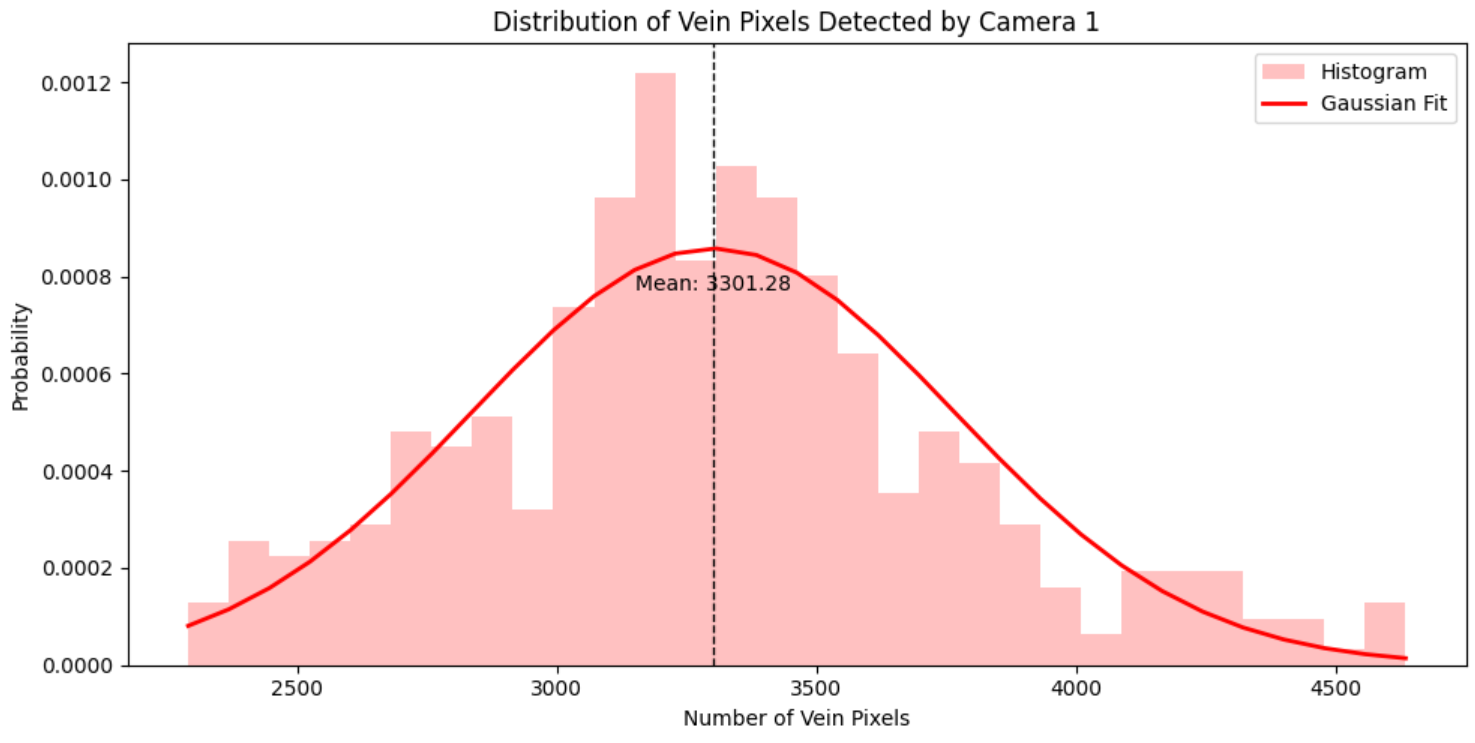
\includegraphics[width=1\linewidth]{latex-img/distribution_veins_cam1.png}
        \caption{Vein Pixel Distribution Analysis Using Camera 1: Histogram Representation with Gaussian Fit Overlay with \(X_i \sim \mathcal{N}(3301.28, 216433.17)\)}
        \label{distribution_veins_cam1}
    \end{figure}

    \begin{figure}[H]
        \centering
        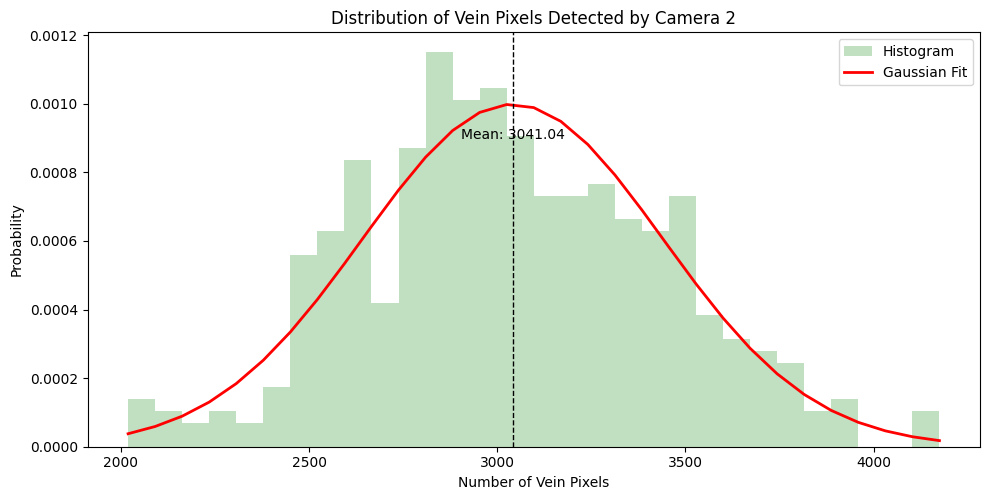
\includegraphics[width=1\linewidth]{latex-img/distribution_veins_cam2.png}
        \caption{Vein Pixel Distribution Analysis Using Camera 2: Histogram Representation with Gaussian Fit Overlay \(X_i \sim \mathcal{N}(3041.04, 159577.13)\)}
        \label{distribution_veins_cam2}
    \end{figure}
 
    \newpage
    \item \textbf{Combined Cameras Distribution}: To understand the aggregate behavior of vein detection across both cameras, the data was merged, generating a comprehensive histogram with a Gaussian fit.

    \begin{figure}[H]
        \centering
        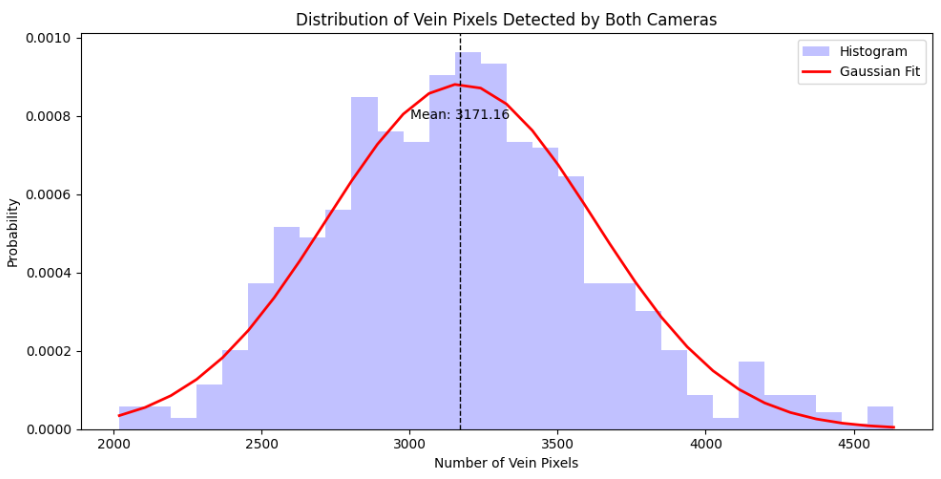
\includegraphics[width=1\linewidth]{latex-img/distribution_veins_bothcams.png}
        \caption{Aggregate Vein Pixel Distribution Analysis: Combined Histogram and Gaussian Fit from Both Cameras \(X_i \sim \mathcal{N}(3171.16, 204935.79)\)}
        \label{distribution_veins_bothcams}
    \end{figure}

\end{enumerate}

Concluding the analysis of the vein pixel distribution across different camera captures and their aggregate dataset, the average probability \(p\) that a given pixel corresponds to a vein was computed. This involved summing up all vein-identifying pixels within the datasets for Camera 1, Camera 2, and the combined dataset. Subsequently, this sum was divided by the total number of pixels processed, multiplying the count of images by the total pixels per image, to ascertain the average likelihood \(p\) that any randomly selected pixel is part of a vein pattern.

The findings from this analysis revealed the following probabilities:
\begin{enumerate}
    \item For Camera 1, the probability \(p^{obs} = \mathbb{E}\left( \frac{\text{HW}(X)}{n} \right)\) was calculated to be \(0.034\), indicating a \(3.42\)\% chance that any given pixel in images from Camera 1 represents a vein.

    \item For Camera 2, the probability \(p^{obs} = \mathbb{E}\left( \frac{\text{HW}(X)}{n} \right)\) was slightly lower at \(0.032\), translating to a \(3.15\)\% chance for vein representation in its images.

    \item When considering the datasets from Both Cameras combined, the probability \(p^{obs} = \mathbb{E}\left( \frac{\text{HW}(X)}{n} \right)\) averaged out to \(0.0329\), suggesting a \(3.29\)\% likelihood of a pixel depicting a vein across the entire dataset. Moreover, the variance (\( \sigma^{2}_p \)) and the standard deviation (\( \sigma_p \)) of the random variable \(\frac{\text{HW}(X)}{n}\) provide insights into the the random variable's spread and consistency. The observed variance is low at approximately \( 2.20 \times 10^{-5} \), indicating minimal fluctuation in the random variables' values among different feature vectors. This suggests that the feature extraction method is highly reliable and consistent across different images. Furthermore, the standard deviation, calculated as approximately \( 4.69 \times 10^{-3} \), reinforces the idea of minimal dispersion around the mean probability (\(p\)) of detecting a vein. 
    
\end{enumerate}

\newpage
\subsection{Experimental Derivation of the Probabilities \(\delta_{\text{same}}, \delta_{\text{diff}}, \delta_{\text{indep}}\)}
\label{sec:delta}

To assess the probability that the i-th pixel of two captures diverges after applying the optimal offset translations \( d_X \) and \( d_Y \) (Equation (\ref{eq:delta})), we undertake additional experimental analysis. This investigation continues to utilize the same dataset comprising 20 distinct individuals. Here, the post-alignment process, specifically Miura Matching, is included in our examination as the calculation formula integrates this step. As detailed in Section~\ref{Bio_data_sim_scores}, our objective is to evaluate three distinct delta values: \(\delta_{\text{same}}, \delta_{\text{diff}}, \delta_{\text{indep}}\). The computation of \( \delta_{\text{indep}} \) is relatively straightforward, having determined the value of \( p \). The formula for \( \delta_{\text{indep}} \) relies solely on \( p \), allowing us to express it as:

\[ \delta_{\text{indep}}^{obs} = 2p^{obs}(1 - p^{obs}) = 2 \times 0.033 \times (1 - 0.033) \approx 6.4\% \]

This result provides an estimated \(6.4\)\% independent delta value.

To accurately evaluate \( \delta_{\text{same}} \) and \( \delta_{\text{diff}} \), a meticulous procedure was executed on our dataset, which involves 20 unique individuals, each having multiple biometric captures. Below is an outline of the methodology applied:

\begin{enumerate}
    \item \textbf{Pairwise Comparison}: For each individual, we compared every biometric capture to every other capture within the dataset, applying the Hamming distance metric to compute the normalized distances.
    \item \textbf{Statistical Analysis}: We organized the resulting distances into two distinct categories:
    \begin{itemize}
        \item Intra-individual distances, where captures from the same individual (same finger images) were compared, forming the first group.
        \item Inter-individual distances, comprising comparisons between biometric captures from different individuals, forming the second group.
    \end{itemize}
    \newpage
    \item \textbf{Probability Computation}:
    \begin{itemize}
        \item For \( \delta_{\text{same}} \), we calculated the average normalized distances from intra-individual comparisons. This analysis provided the following results, quantifying the observed differences between captures from the same individual after alignment:

        \[ \delta_{\text{same}}^{obs} \approx 4.55\% \]
        \[ \sigma_{\delta_{same}} \approx 1.03 \times 10^{-2} \]
        \[ \sigma²_{\delta_{same}} \approx 1.06 \times 10^{-4} \]

        \begin{figure}[H]
            \centering
            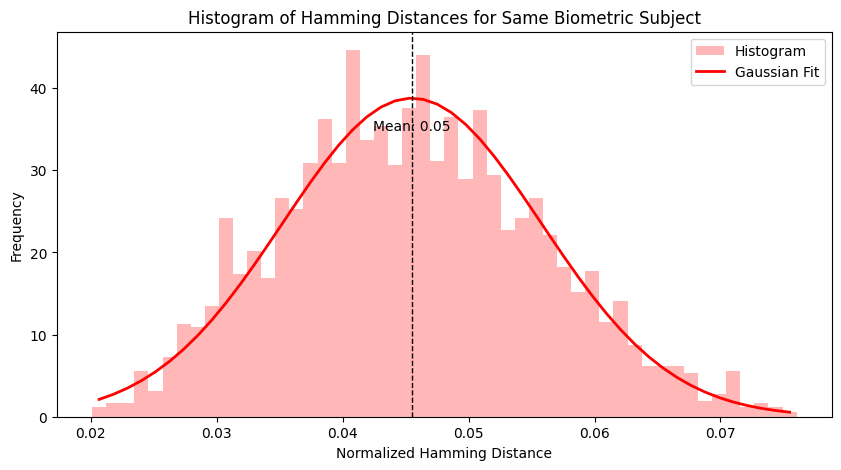
\includegraphics[width=0.7\linewidth]{latex-img/delta_same.png}
            \caption{Frequency Distribution of Normalized Hamming Distances for Identical Biometric Samples with Alignment \(\delta_{same} \sim \mathcal{N}(0.045, 0.000106)\)}
            \label{delta_same}
        \end{figure}
        
        \item For \( \delta_{\text{diff}} \), we performed a similar averaging of the normalized distances from the inter-individual comparisons, which furnished us with the following results for observing a difference between captures from the different individuals after alignment:

        \[ \delta_{\text{diff}}^{obs} \approx 5.99\% \]
        \[ \sigma_{\delta_{diff}} \approx 6.76 \times 10^{-3} \]
        \[ \sigma²_{\delta_{diff}} \approx 4.58 \times 10^{-5} \]

        \begin{figure}[H]
            \centering
            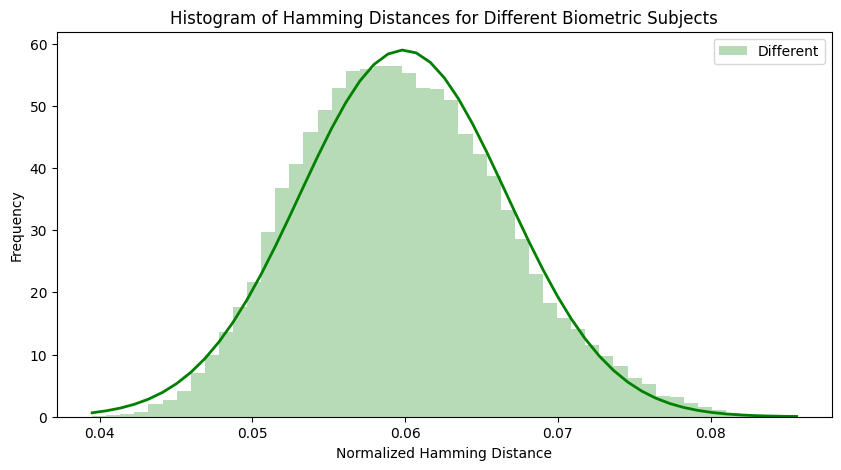
\includegraphics[width=0.7\linewidth]{latex-img/delta_diff.png}
            \caption{Frequency Distribution of Normalized Hamming Distances for Different Biometric Samples with Alignment \(\delta_{diff} \sim \mathcal{N}(0.0599, 0.0000458)\)}
            \label{delta_diff}
        \end{figure}
    \end{itemize}
\end{enumerate}

The joint probability distribution presented in Table \ref{tab:joint_distribution} represents the relationship between the variables \(\bar{X}_i\) and \(\bar{Y}_i\), which compare the i-th bit of two biometric samples. The parameter \(p\) denotes the probability of a bit being '1', and by complement, \(1-p\) signifies the probability of a bit being '0'. The parameter \(\delta\) encapsulates the probability that the two bits are not identical, which can occur due to various sources of error in biometric comparison. 

In Table \ref{tab:joint_distribution}, we explain each entry:

\begin{itemize}
    \item By utilizing the previously determined value of $\delta$, we can infer the probabilities \(P[\bar{X}_i = 1, \bar{Y}_i = 0]\) and \(P[\bar{X}_i = 0, \bar{Y}_i = 1]\) as follows: 
    \begin{equation*}
        \begin{aligned}
            \delta = P[\bar{X}_i \neq \bar{Y}_i] = P[\bar{X}_i = 1, \bar{Y}_i = 0] + P[\bar{X}_i = 0, \bar{Y}_i = 1]
        \end{aligned}
    \end{equation*}
    Hence we have:
    \begin{equation*}
        \begin{aligned}
            P[\bar{X}_i = 1, \bar{Y}_i = 0] = P[\bar{X}_i = 0, \bar{Y}_i = 1] = \frac{\delta}{2}
        \end{aligned}
    \end{equation*}
    \item To determine the probability\(P[\bar{X}_i = 0, \bar{Y}_i = 0]\), we consider the following relationships and utilize the law of total probability:
    \begin{equation*}
        \begin{aligned}
            P[\bar{X}_i = 0] = 1-p = P[\bar{X}_i = 0, \bar{Y}_i = 0] + P[\bar{X}_i = 0, \bar{Y}_i = 1]
        \end{aligned}
    \end{equation*} 
    \begin{equation*}
        \begin{aligned}
            P[\bar{Y}_i = 0] = 1-p = P[\bar{X}_i = 0, \bar{Y}_i = 0] + P[\bar{X}_i = 1, \bar{Y}_i = 0]
        \end{aligned}
    \end{equation*} 
    
    By solving these equations, we can derive the probability of interest, \\\(P[\bar{X}_i = 0, \bar{Y}_i = 0]\), and hence infer the previously obtained values for \\\(P[\bar{X}_i = 1, \bar{Y}_i = 0]\) and \(P[\bar{X}_i = 0, \bar{Y}_i = 1]\):
    \[ P[\bar{X}_i = 0, \bar{Y}_i = 0] = 1-p - \frac{\delta}{2} \] 

    \item The probability \(P[\bar{X}_i = 1, \bar{Y}_i = 1]\) is derived by 
    \[P[\bar{X}_i = 1, \bar{Y}_i = 1] = 1 - P[\bar{X}_i = 0, \bar{Y}_i = 0] = p-\frac{\delta}{2}\]

\end{itemize}

Utilizing \(\delta_{same}^{obs}\), \(\delta_{diff}^{obs}\) and \(\delta_{indep}^{obs}\), we can determine the corresponding probabilities presented in Table \ref{tab:joint_distribution}. This gives us the following figures:

\begin{table}[H]
    \centering
    \renewcommand{\arraystretch}{1.5}
    \begin{tabular}{|c|c|c|}
        \hline
        & $\bar{Y}_i = 0$ & $\bar{Y}_i = 1$\\
        \hline
        $\bar{X}_i = 0$ & $1 - p - \frac{\delta_{indep}^{obs}}{2} = 93.5\% $ & $\frac{\delta_{indep}^{obs}}{2} = 3.2\%$\\
        \hline
        $\bar{X}_i = 1$ & $\frac{\delta_{indep}^{obs}}{2} = 3.2\% $ & $p - \frac{\delta_{indep}^{obs}}{2} = 0.1\%$\\
        \hline
    \end{tabular}
    \caption{Joint Distribution of ($\bar{X}_j$, $\bar{Y}_j$) for \(X\) and \(Y\) made up of \(2n\) independent random bits of expected value \(p\)}
    \label{tab:joint_distribution_deltaindep}
\end{table}


\begin{table}[H]
    \centering
    \renewcommand{\arraystretch}{1.5}
    \begin{tabular}{|c|c|c|}
        \hline
        & $\bar{Y}_i = 0$ & $\bar{Y}_i = 1$\\
        \hline
        $\bar{X}_i = 0$ & $1 - p - \frac{\delta_{same}^{obs}}{2} = 94.4\% $ & $\frac{\delta_{same}^{obs}}{2} = 2.3\%$\\
        \hline
        $\bar{X}_i = 1$ & $\frac{\delta_{same}^{obs}}{2} = 2.3\%$ & $p - \frac{\delta_{same}^{obs}}{2} = 1\%$\\
        \hline
    \end{tabular}
    \caption{Joint Distribution of ($\bar{X}_j$, $\bar{Y}_j$) for \(X\) and \(Y\)  Originating from the Same Biometric Subject}
    \label{tab:joint_distribution_deltasame}
\end{table}

\begin{table}[H]
    \centering
    \renewcommand{\arraystretch}{1.5}
    \begin{tabular}{|c|c|c|}
        \hline
        & $\bar{Y}_i = 0$ & $\bar{Y}_i = 1$\\
        \hline
        $\bar{X}_i = 0$ & $1 - p - \frac{\delta_{diff}^{obs}}{2} = 93.7\% $ & $\frac{\delta_{diff}^{obs}}{2} = 3\%$\\
        \hline
        $\bar{X}_i = 1$ & $\frac{\delta_{diff}^{obs}}{2} = 3\%$ & $p - \frac{\delta_{diff}^{obs}}{2} = 0.3\%$\\
        \hline
    \end{tabular}
    \caption{Joint Distribution of ($\bar{X}_j$, $\bar{Y}_j$) for \(X\) and \(Y\) Originating from Different Biometric Subject}
    \label{tab:joint_distribution_deltadiff}
\end{table}










\section{Fuzzy Hashing}
\label{sec:Fuzzy Hashing}
Fuzzy hashing, as opposed to traditional hashing, produces consistent cryptographic keys for similar but not identical inputs, enabling recognition of the same biometric trait across different instances despite slight variations. This approach ensures legitimate users are not incorrectly denied access due to minor discrepancies and protects user privacy by storing and using hashed values instead of raw biometric data, making it difficult to reverse-engineer the original data even if unauthorized access occurs. 
This section will discuss how we implemented the fuzzy hashing algorithm, its corresponding mathematical aspects and some experiments.

\subsection{PreHash Algorithm}

The preHash algorithm is the first step in the fuzzy hashing process, designed to manipulate biometric templates extracted from finger vein patterns. It operates on a bitstring \(X\), representing the presence (1) or absence (0) of vein pixels across \(n\) pixels, where \(n=90'240\).

Algorithm Inputs and Outputs:
\begin{enumerate}
    \item \textbf{Inputs}: As illustrated in the pseudocode~\ref{preHash Algorithm}, the algorithm takes three main inputs:
    \begin{itemize}
        \item \textbf{A parameter m}: the number of indices to find
        \item \textbf{A bitstring X}: the feature-extracted vein patterns of a biometric capture
        \item \textbf{A key}: used to initialize a Pseudorandom Number Generator (PRNG)
    \end{itemize}
    \item \textbf{Output}: The algorithm outputs a tuple \((i_1,...,i_m)\) consisting of the \(m\) smallest indices \(i_j\)​ such that \(1 \leq i_1<...<i_m\)​ and the pixel at \(PRNG_{key(i_j)}\) in \(X\) is identified as a vein pixel. 
\end{enumerate}

Detailed Process of preHash:
\begin{itemize}
    \item \textbf{Initiallization}: Utilizing the provided key, the algorithm initializes a PRNG. This PRNG is based on the \hyperref[def:AES CTR mode]{Advanced Encryption Standard (AES) in Counter (CTR) mode}, ensuring the generation of uniform and independent pseudorandom sequences.

    \item \textbf{Nonce Generation}: A nonce in CTR mode encryption is initialized to zero to maintain simplicity and security. We opted against using a keyed hash function to generate the nonce, as it would tie the nonce to the secret key. Such a dependency would mean that both the nonce and the Pseudo-Random Number Generator (PRNG) would rely on the same key, creating a security risk by concentrating security on a single element. To avoid this, we keep the generation of the nonce separate from the key.

    \item \textbf{Pseudorandom Sequence Generation}: Upon initialization with the specified parameters—key and nonce—the PRNG operates in Counter (CTR) mode to generate a sequence of pseudo-random numbers. As illustrated in Figure~\ref{ctr encryption}, the process involves encrypting an incrementing counter combined with the nonce using the specified key. The output from this block cipher encryption is used to generate a unique stream of pseudo-random bits.
    To optimize the utilization of the cryptographic output and reduce operational overhead, the PRNG is designed to generate a full 128-bit block of pseudo-random data at a time, even though only a portion of these bits are used immediately. When a new block is generated, the algorithm extracts the lowest 17 bits to obtain the pseudo-random number for the current operation. This choice is aligned with the project's requirement for representing image sizes, where a maximum of \(90'240\) pixels can be represented, necessitating exactly 17 bits per operation (\(\left\lceil \log_2(90'240) \right\rceil = 17\)). These extracted bits serve as the pseudo-random number.
    Following extraction, the algorithm discards the used bits from the current block by right-shifting the block by 17 bits. This operation updates the state of the PRNG, ensuring that the consumed bits are no longer considered in subsequent operations. In the case where there are no longer 17 bits available after extraction, the algorithm generates a new pseudo-random number using the PRNG and repeats the process. This mechanism guarantees the efficient utilization of all bits produced by the block cipher, enhancing efficiency and reducing operational overhead.
    The predictability and reproducibility of the sequence are entirely dictated by the chosen key. Employing the same key across sessions guarantees the generation of an identical sequence of pseudo-random numbers.
    
     

    \begin{figure}[!h]
        \centering
        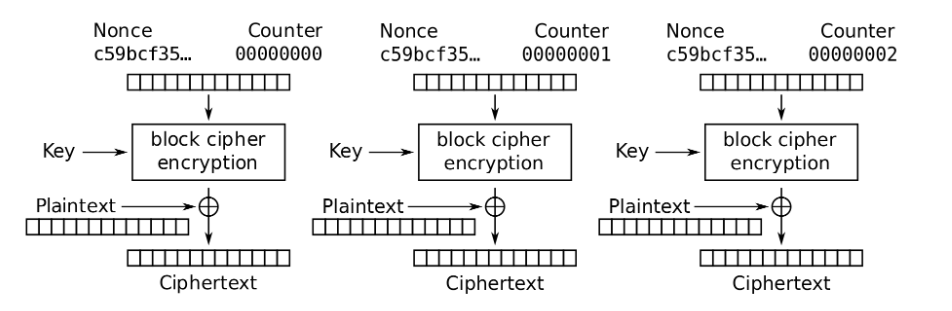
\includegraphics[width=1\linewidth]{latex-img/CTR_encryption.png}
        \caption{Counter (CTR) mode encryption}
        \label{ctr encryption}
    \end{figure}
    

    \item \textbf{Selection of Indices}: The algorithm iterates through the generated pseudorandom sequence, selecting the first \(m\) indices corresponding to vein pixels in the biometric template \(X\). This selection process involves a careful mechanism to ensure the uniqueness and proper ordering of indices.

    \item \textbf{Corner Cases}: In scenarios where there are no veins present in the image, the algorithm incorporates a built-in mechanism to address such situations. Prior to initiating the preHash process, it assesses whether at least one vein is present in the image. If no veins are detected, the algorithm suspends further execution, preventing an infinite loop.

\end{itemize}


\begin{algorithm}
\begin{algorithmic}[1]
\caption{preHash Algorithm}
\label{preHash Algorithm}
\Function{preHash$_\text{key}^m$}{$X$}
\State \hfill $\triangleright$ $L \gets \lceil \log_2(n) \rceil$
\State Initialize PRNG using key for $L$ bits
\State $i \gets 0$
\For{$j \gets 1 \text{ to } m$}
    \Repeat
        \Repeat
            \State $k \gets \text{PRNG}$
        \Until{$1 \leq k \leq n$}
        \State $i \gets i + 1$
    \Until{$X_k$ is a vein pixel}
    \State $i_j \gets k$
    \EndFor 
\State \Return{$i_1, \ldots, i_m$}
\EndFunction
\end{algorithmic}
\end{algorithm}

The algorithm, preHash, illustrated in Figure~\ref{preHash Algorithm} generates \(m\) smallest indices, denoted by \(i_j\), such that \(j\in{[1, m]} \) and \(1 \leq i_1 < ... < i_m\), where each \(i_j\) correponds to an index such that \(X_{PRNG_{key}(i_j)} = 1\). It achieves this by rigorously verifying that the numbers produced by PRNG stay within the specified bounds, i.e. \(\text{PRNG}[i] \in (0, n] \text{ for all } i \in [0, m]\).

\subsection{Assessing Similarity of Biometric Inputs After PreHash Application}
\label{sec:mu}

After the finger images are processed through the pipeline described in Figure~\ref{pipeline_simon} to extract their feature vectors, and the preHash algorithm is applied, the outcome is a set of indices that fall within the inclusive range \(\text{PRNG}[i] \in (0, n] \text{ for } i \in [0, m]\), effectively mapping each selected feature to a unique index within the feature vector's length.

In the context of a simplified scenario where the hash length parameter (\(m\)) is set to \(1\), implying the generation of a single-index hash, and assuming a randomly chosen key for the preHash algorithm, along with \(k\) representing a uniformly distributed random index, the probability that the preHash operation yields the same index for two different fixed inputs \(X\) and \(Y\) can be mathematically delineated as follows:


\begin{equation} \label{eq:preHash1}
    \begin{aligned}
        Pr[preHash_{key}^1(X) = preHash_{key}^1(Y)] &= \sum_{i > 0} Pr[preHash_{key}^1(X) = preHash_{key}^1(Y) = i]\\
        &= \sum_{i > 0} Pr[X_k = Y_k = 0]^{i - 1} Pr[X_k = Y_k = 1]\\
        &= \frac{Pr[X_k = Y_k = 1]}{1 - Pr[X_k = Y_k = 0]}\\
        &= \frac{HW(X \land Y)}{HW(X) + HW(Y) - HW(X \land Y)}\\
        &= \frac{1}{\frac{1}{Score(X, Y)} - 1}
    \end{aligned}
\end{equation}

This equation encapsulates the likelihood of two images, \(X\) and \(Y\), having their singular hash index coincide, based on the presence of matching features identified by the algorithm. The final form of the equation relates the probability to the scoring function between \(X\) and \(Y\), inversely proportional to the score minus one.

It is noticed that there is a direct link with the Miura matching score that is of interest. The direct link between the preHash algorithm's outcomes and the Miura matching score lies in their shared foundation of evaluating biometric similarities. Specifically, both methodologies utilize Hamming weight and bitwise operations to assess the overlap between biometric samples, such as finger vein patterns. The preHash algorithm, through its probabilistic formula, quantifies the likelihood of matching indices based on feature presence, closely paralleling the Miura score's approach of comparing binary patterns to derive a similarity score. The above computation can also be expressed as follows:

\begin{equation} \label{eq:preHash2}
    \begin{aligned}
        Pr[preHash_{key}^1(\bar{X}) = preHash_{key}^1(\bar{Y})] &= \frac{Pr[\bar{X}_k = \bar{Y}_k = 1]}{1 - Pr[\bar{X}_k = \bar{Y}_k = 0]}\\
        &= \frac{\frac{Pr[X_k = 1] + Pr[Y_k = 1]}{2} - \frac{1}{2}Pr[\bar{X}_k \neq \bar{Y}_k]}{\frac{Pr[X_k = 1] + Pr[Y_k = 1]}{2} + \frac{1}{2}Pr[\bar{X}_k \neq \bar{Y}_k]}\\
    \end{aligned}
\end{equation}

The following approximations are made, inspired by equations \(p\) (\ref{eq:p}) and $\delta$ (\ref{eq:delta}):

\begin{equation}
    \mathbb{E}\left(\frac{\frac{Pr[X_k = 1] + Pr[Y_k = 1]}{2} - \frac{1}{2}Pr[\bar{X}_k \neq \bar{Y}_k]}{\frac{Pr[X_k = 1] + Pr[Y_k = 1]}{2} + \frac{1}{2}Pr[\bar{X}_k \neq \bar{Y}_k]}\right) \approx \frac{p - \frac{\delta}{2}}{p + \frac{\delta}{2}}
\end{equation}

The core of this approximation revolves around the expectation formula, which integrates probabilities of feature presence \(Pr[X_k=1]+Pr[Y_k=1]\) and the likelihood of discrepancies between \(\bar{X}\) and \(\bar{Y}\), \(Pr[\bar{X}_k \neq \bar{Y}_k]\). This formula essentially aims to quantify the similarity between two biometric samples by considering both the concurrence of features and the instances where they diverge.

To achieve a more accurate approximation of the expected value of Equation \ref{eq:preHash2}, we define the following parameters and employ a Taylor series expansion of the function \(f(A,B,C) = \frac{A + B - C}{A + B + C}\) around the point \((p, p, \delta)\). This method allows us to incorporate not only the means but also the variances and covariances of the variables involved.

\[
A = \frac{HW(\bar{X})}{n}, \quad B = \frac{HW(\bar{Y})}{n}, \quad C = \frac{d_H(\bar{X}, \bar{Y})}{n}
\]
where \(HW(\cdot)\) denotes the Hamming weight and \(\frac{d_H(\cdot, \cdot)}{n}\) represents the normalized Hamming distance. Given these definitions, we know the expected values and variances from Section~\ref{sec:bio_setting} :
\[
    \mathbb{E}(A) = \mathbb{E}(B) = p^\text{obs}, \quad \mathbb{E}(C) = \delta^\text{obs}, \quad \mathbb{V}(A) = \mathbb{V}(B) = ({\sigma^\text{obs}_p})^2, \quad \mathbb{V}(C) = ({\sigma^\text{obs}_\delta})^2
\]

Next, we perform a Taylor series expansion of \(f(A,B,C)\) up to the second order around the point \((p, p, \delta)\). The first-order partial derivatives are calculated as follows:
\[
f'_A = \frac{2C}{(A + B + C)^2}, \quad f'_B = \frac{2C}{(A + B + C)^2}, \quad f'_C = \frac{-2(A + B)}{(A + B + C)^2}
\]

The second-order partial derivatives are:
\[
f''_{AA} = f''_{BB} = f''_{AB} = \frac{-4C}{(A + B + C)^3}, \quad f''_{CC} = \frac{4(A + B)}{(A + B + C)^3}, \quad f''_{AC} = f''_{BC} = \frac{-2(A + B - C)}{(A + B + C)^3}
\]

By substituting \(A = p\), \(B = p\), and \(C = \delta\) into these second order derivatives, we obtain:

\[
f''_{AA} = f''_{BB} = f''_{AB} = \frac{-4\delta}{(2p + \delta)^3}, \quad f''_{CC} = \frac{8p}{(2p + \delta)^3}, \quad f''_{AC} = f''_{BC} = \frac{2(2p - \delta)}{(2p + \delta)^3}
\]

Finally, the second order Taylor expansion of \(f(A,B,C)\) around \((p,p,\delta)\) is given by:
\[
f(A,B,C) \approx f(p,p,\delta) + f'_A(p,p,\delta)(A - p) + f'_B(p,p,\delta)(B - p) + f'_C(p,p,\delta)(C - \delta)
\]
\[
+ \frac{1}{2} \left[ f''_{AA}(p,p,\delta)(A - p)^2 + f''_{BB}(p,p,\delta)(B - p)^2 + f''_{CC}(p,p,\delta)(C - \delta)^2 \right.
\]
\[
+ 2f''_{AB}(p,p,\delta)(A - p)(B - p) + 2f''_{AC}(p,p,\delta)(A - p)(C - \delta) + 2f''_{BC}(p,p,\delta)(B - p)(C - \delta)
\]\\
To approximate the expected value \( E(f(A,B,C)) \), we use the following relations:
\[
    \mathbb{E}(A - p) = 0, \quad \mathbb{E}(B - p) = 0, \quad \mathbb{E}(C - \delta) = 0
\]
\[
    \mathbb{V}(A) = \mathbb{V}(B) = \mathbb{E}((A - p)²), \quad \mathbb{V}(C) = \mathbb{E}((C - \delta)²)
\]
\[
    \text{Cov}(A, B) = \mathbb{E}((A - p)(B - p)), \quad \text{Cov}(B, C) = \mathbb{E}((B - p)(C - \delta))
\]
\[
    \text{Cov}(A, C) = \mathbb{E}((A - p)(C - \delta))
\]

And we hence have:
\[
    \mathbb{E}(f(A,B,C)) \approx \frac{p - \frac{\delta}{2}}{p + \frac{\delta}{2}} + \frac{1}{2} \left[ f''_{AA}(p,p,\delta)\mathbb{V}(A) + f''_{BB}(p,p,\delta)\mathbb{V}(B) + f''_{CC}(p,p,\delta)\mathbb{V}(C) \right.
\]
\[
+ 2f''_{AB}(p,p,\delta) \text{Cov}(A,B) + 2f''_{AC}(p,p,\delta) \text{Cov}(A,C) + 2f''_{BC}(p,p,\delta) \text{Cov}(B,C)]
\]

Simplifying with our values and notations we get:

\begin{equation}
    \begin{aligned}
    \mathbb{E}(f(A,B,C)) &\approx \frac{p - \frac{\delta}{2}}{p + \frac{\delta}{2}} + \frac{1}{2} \left[ \frac{-4\delta}{(2p + \delta)^3}\cdot({\sigma^\text{obs}_p})^2 + \frac{-4\delta}{(2p + \delta)^3}\cdot({\sigma^\text{obs}_p})^2 \right. \\[2mm]
    & \left. + \frac{8p}{(2p + \delta)^3}\cdot({\sigma^\text{obs}_\delta})^2 + 2\cdot\frac{-4\delta}{(2p + \delta)^3}\cdot\text{Cov}(A,B) \right. \\[2mm]
    & \left. + 2\cdot\frac{2(2p - \delta)}{(2p + \delta)^3}\cdot\text{Cov}(A,C) + 2\cdot\frac{2(2p - \delta)}{(2p + \delta)^3}\cdot\text{Cov}(B,C) \right]\\
    \end{aligned}
    \label{eq:mu_approximation}
\end{equation}

Hence for (\(X\), \(Y\)) random,
\begin{equation}
    \label{eq:mu_leq}
    Pr[preHash_{key}^1(offset_X * X) = preHash_{key}^1(offset_Y * Y)] \leq \mathbb{E}(f(A,B,C))
\end{equation}
where equality is reached for the optimal offset translations.\\

Depending on the distribution of (\(X\), \(Y\)), it is denoted

\begin{equation} \label{eq:mu}
    \mu = \mathbb{E}(f(A,B,C))
\end{equation}\\

In order to assess the theoretical approximations of $\mu_{same}$, $\mu_{diff}$, and the value of $\mu_{indep}$, we can easily replace the different values in Equation~\ref{eq:mu_approximation} with the corresponding values calculated in the previous sections. We demonstrate how this is done for \( \mu_{\text{indep}}^{obs} \). Using \( p^{obs} \), \(\delta_{\text{indep}}^{obs}\), and their respective standard deviations, we aim to calculate \(\mathbb{E}(f(A,B,C))\). This calculation is based on \(X\) and \(Y\) comprising \(2n\) independent random bits with an expected value of \(p\), without applying the optimal offset to obtain \(\bar{X}\) and \(\bar{Y}\). Equation~\ref{eq:mu_approximation} is simplified because the covariance between \(A\) and \(B\) is zero (because of independence).

For clarity, note that in the following equation:

- \(p\) corresponds to \(p^{obs}\),\\
- \(\delta\) corresponds to \(\delta_{\text{indep}}^{obs}\),\\
- \(\sigma_p\) corresponds to \(\sigma_p^{obs}\), and\\
- \(\sigma_\delta\) corresponds to \(\sigma_{\delta_{\text{indep}}}^{\text{obs}}\).

This allows us to express \( \mu_{\text{indep}}^{obs} \) as follows:

\begin{equation}
    \begin{aligned}
    \mu_{\text{indep}}^{obs} = \mathbb{E}(f(A,B,C)) &\approx \quad \frac{p - \frac{\delta}{2}}{p + \frac{\delta}{2}} + \frac{1}{2} \left[ \frac{-4\delta}{(2p + \delta)^3}\cdot({\sigma^\text{obs}_p})^2 + \frac{-4\delta}{(2p + \delta)^3}\cdot({\sigma^\text{obs}_p})^2 \right. \\[2mm]
    & \left. + \frac{8p}{(2p + \delta)^3}\cdot({\sigma^\text{obs}_\delta})^2 + 2\cdot\frac{2(2p - \delta)}{(2p + \delta)^3}\cdot\text{Cov}(A,C) \right. \\[2mm]
    & \left. + 2\cdot\frac{2(2p - \delta)}{(2p + \delta)^3}\cdot\text{Cov}(B,C) \right]\\[6mm]
    & = \num{1.78e-2} + \frac{1}{2} \left[ -2\cdot\num{2.6e-3} + \num{1.5e-4}  \right. \\[2mm]
    & \left. + 2\cdot\num{1.31e-6} \right] \\[6mm]
    & \approx 0.01536 = 1.54\%
    \end{aligned}
    \label{eq:mu_indep}
\end{equation}\\

We proceed in a similar way to assess the theoretical values of $\mu_{same}$ and $\mu_{diff}$, except in this case the covariances are non-zero and have been calculated by observing the correlation between the different random variables (\(A\), \(B\), \(C\)) in the experimental results obtained in Section~\ref{sec:bio_setting}. That is, we calculated the covariance matrix between the following random variables:
\[
A = \frac{HW(\bar{X})}{n}, \quad B = \frac{HW(\bar{Y})}{n}, \quad C = \frac{d_H(\bar{X}, \bar{Y})}{n}
\]

We obtained the following covariance matrices from the experiments held to find \(\delta^{obs}_{diff}\) and \(\delta^{obs}_{same}\):

\[
\begin{array}{c|ccc}
           & \text{A} & \text{B} & \text{C} \\
\hline
\text{A} & 0.000025 & 0.000022 & 0.000036 \\
\text{B} & 0.000022 & 0.000025 & 0.000036 \\
\text{C} & 0.000036 & 0.000036 & 0.000106 \\
\end{array}
\]
\begin{center}\text{Covariance Matrix for Same Distribution}\end{center}


\[
\begin{array}{c|ccc}
           & \text{A} & \text{B} & \text{C} \\
\hline
\text{A} & 0.000025 & 0.000006 & 0.000026 \\
\text{B} & 0.000006 & 0.000026 & 0.000027 \\
\text{C}  & 0.000026 & 0.000027 & 0.000046 \\
\end{array}
\]
\begin{center}\text{Covariance Matrix for Different Distribution}\end{center}

We have the following equations for \(\mu_{same}\) and \(\mu_{diff}\). Depending on the distribution (same or different), the variables \(p\), \(\delta\), \(\sigma_p\), and \(\sigma_\delta\) correspond to their observed counterparts as indicated:

- \(p \rightarrow p^{obs}\)\\
- \(\delta \rightarrow \delta_{\text{same/diff}}^{obs}\)\\
- \(\sigma_p \rightarrow \sigma_p^{obs}\)\\
- \(\sigma_\delta \rightarrow \sigma_{\delta_{\text{same/diff}}}^{\text{obs}}\)\\

\begin{equation}
    \begin{aligned}
    \mu_{\text{same}}^{obs} = \mathbb{E}(f(A,B,C)) &\approx \quad \frac{p - \frac{\delta}{2}}{p + \frac{\delta}{2}} + \frac{1}{2} \left[ \frac{-4\delta}{(2p + \delta)^3}\cdot({\sigma^\text{obs}_p})^2 + \frac{-4\delta}{(2p + \delta)^3}\cdot({\sigma^\text{obs}_p})^2 \right. \\[2mm]
    & \left. + \frac{8p}{(2p + \delta)^3}\cdot({\sigma^\text{obs}_\delta})^2 + 2\cdot\frac{-4\delta}{(2p + \delta)^3}\cdot\text{Cov}(A,B) \right. \\[2mm] 
    & \left. + 2\cdot\frac{2(2p - \delta)}{(2p + \delta)^3}\cdot\text{Cov}(A,C) + 2\cdot\frac{2(2p - \delta)}{(2p + \delta)^3}\cdot\text{Cov}(B,C) \right]\\[10mm]
    & = \num{2.14e-1} + \frac{1}{2} \left[ -2\cdot\num{2.9e-3} + \num{1.9e-2}  \right. \\[2mm]
    & \left. - \num{5.1e-3} + 2\cdot\num{2.3e-3} \right] \\[10mm]
    & \approx 0.22048 = 22.05\%
    \end{aligned}
    \label{eq:mu_same}
\end{equation}

\begin{equation}
    \begin{aligned}
    \mu_{\text{diff}}^{obs} = \mathbb{E}(f(A,B,C)) &\approx \quad \frac{p - \frac{\delta}{2}}{p + \frac{\delta}{2}} + \frac{1}{2} \left[ \frac{-4\delta}{(2p + \delta)^3}\cdot({\sigma^\text{obs}_p})^2 + \frac{-4\delta}{(2p + \delta)^3}\cdot({\sigma^\text{obs}_p})^2 \right. \\[2mm]
    & \left. + \frac{8p}{(2p + \delta)^3}\cdot({\sigma^\text{obs}_\delta})^2 + 2\cdot\frac{-4\delta}{(2p + \delta)^3}\cdot\text{Cov}(A,B) \right. \\[2mm] 
    & \left. + 2\cdot\frac{2(2p - \delta)}{(2p + \delta)^3}\cdot\text{Cov}(A,C) + 2\cdot\frac{2(2p - \delta)}{(2p + \delta)^3}\cdot\text{Cov}(B,C) \right]\\[10mm]
    & = \num{7.99e-2} + \frac{1}{2} \left[ -2\cdot\num{2.7e-3} + \num{5.8e-3}  \right. \\[2mm]
    & \left. - \num{1.3e-3} + \num{4.9e-4} + \num{5e-4} \right] \\[10mm]
    & \approx 0.07993 = 7.99\%
    \end{aligned}
    \label{eq:mu_diff}
\end{equation}

Finally, the following figures are provided:

\begin{table}[H]
    \centering
    \renewcommand{\arraystretch}{1.25}\begin{tabular}{|c|c|c|}
        \hline
        $\mu_{same}$ & $\mu_{diff}$ & $\mu_{indep}$\\
        \hline
        $21.41\%$ & $7.99\%$ & $1.78\%$\\
        \hline
    \end{tabular}
\caption{Theoretical Approximations without Taylor Series Expansion: $\mu_{same}$, $\mu_{diff}$, and $\mu_{indep}$}
\label{tab:mu_approx}
\end{table}


\begin{table}[H]
    \centering
    \renewcommand{\arraystretch}{1.25}\begin{tabular}{|c|c|c|}
        \hline
        $\mu_{same}$ & $\mu_{diff}$ & $\mu_{indep}$\\
        \hline
        $22.05\%$ & $7.99\%$ & $1.54\%$\\
        \hline
    \end{tabular}
\caption{Theoretical Approximations with Taylor Series Expansion: $\mu_{same}$, $\mu_{diff}$, and $\mu_{indep}$}
\label{tab:approximation_mu_taylor}
\end{table}

We can note that there is not a major difference between approximations from Table~\ref{tab:approximation_mu_taylor} and Table~\ref{tab:mu_approx}. Yet, the approximation from Table~\ref{tab:approximation_mu_taylor} yields extremely close values to the experimental results from subsection~\ref{sec:experiment_fuzzy_hash}.

Finally, it is observed that:

\begin{equation}
    Pr[preHash_{key}^m(offset_X * X) = preHash_{key}^m(offset_Y * Y)] \leq \mu^m
\end{equation}
\\
where equality is reached for the optimal offset translations.

\subsection{Experimental Derivation of the Probabilities \(\mu_{\text{same}}^{\text{obs}}, \mu_{\text{diff}}^{\text{obs}}, \mu_{\text{indep}}^{\text{obs}}\)}
\label{sec:experiment_fuzzy_hash}

In Section~\ref{sec:mu}, we have laid out the mathematical framework that defines the upper bound \(\mu\). This probability is crucial in our fuzzy hashing approach, as it quantifies the matching likelihood after applying the optimal offset translations to the biometric captures. The application of these optimal offsets is an important preprocessing step before hashing the dataset, ensuring that the biometric features are accurately aligned for comparison.

We will proceed to evaluate these theoretical approximations (Table~\ref{tab:mu_approx}) experimentally, leveraging the same comprehensive database that has been utilized in our prior research, as explained in Section~\ref{sec:delta}. This experimental assessment will enable us to substantiate the theoretical predictions of \(\mu_{\text{same}}\) and \(\mu_{\text{diff}}\).

In the experimental setup, \(\mu^{obs}_{\text{same}}\) refers to the probability that a hash function, when applied to two biometric captures of the same finger, will yield the same index. This is the measure of success in correctly identifying matches within the same individual's biometric captures. Conversely, \(\mu^{obs}_{\text{diff}}\) denotes the probability that the same hash function will produce different indices for biometric captures from different individuals, representing the ability to distinguish between different people's biometric data. Lastly, \(\mu^{obs}_{\text{indep}}\) indicates the probability of a match in the case where the biometric captures are completely independent, serving as a baseline for random chance, which has already been calculated (see Equation~\ref{eq:mu_indep})

For \(\mu_{\text{same}}^{obs}\) and \(\mu_{\text{diff}}^{obs}\), our experimental protocol adhered to the established optimal pipeline (refer to Figure~\ref{pipeline_simon}) to process the images in our dataset. Following the alignment of images through the computation of optimal offsets (referred to as Miura Matching), our fuzzy hashing function was applied to the extraced features. In alignment with the premise that \(\mu\) is computed under the condition where the hash function's output is a single index (\(m=1\)).

\begin{enumerate}
    \item \textbf{Pairwise Comparison}: We performed a pairwise comparison for each image pair within the dataset after applying the optimal offsets to ensure proper alignment. The fuzzy hashing function, tailored to output a single index per image, was utilized to hash the images.

    \item \textbf{Hamming Distance Computation}: We calculated the Hamming distance between the indices obtained from the fuzzy hashing. The distances were binary:
    \begin{itemize}
        \item A Hamming distance of 0 indicates the indices are identical, suggesting a match.
        \item A Hamming distance of 1 indicates differing indices, suggesting a non-match.
    \end{itemize} 
    
    \item \textbf{Statistical Analysis and Probability Computation}:
    \begin{itemize}
        \item \textbf{\(\mu_{\text{same}}^{obs}\)}: We computed \(\mu_{\text{same}}^{obs}\) by averaging the number of Hamming distances that resulted in a match (Hamming distances of 0) of the intra-individual comparisons, which furnished us with the following probability:

        \[ \mu_{\text{same}}^{obs} \approx 0.22047 = 22.05\%\]
        
        \item \textbf{\(\mu_{\text{diff}}^{obs}\)}: Similarly, \(\mu_{\text{diff}}^{obs}\) was determined by averaging the number of Hamming distances that resulted in a match (Hamming distances of 0) of the inter-individual comparisons, which furnished us with the following probability:

        \[ \mu_{\text{diff}}^{obs} \approx 0.08249 = 8.25\% \]
        \begin{figure}[H]
            \centering
            \begin{subfigure}[b]{0.48\linewidth}
                \centering
                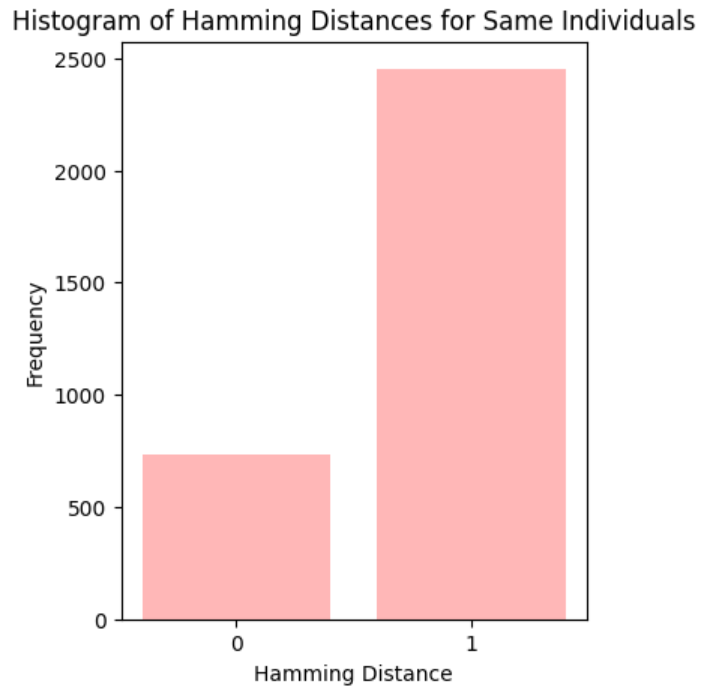
\includegraphics[width=\linewidth,height=7cm,keepaspectratio]{latex-img/mu_same.png}
                \caption{Count of the number of matches for Same, Aligned Biometric Samples with Single Index preHashing}
                \label{mu_same}
            \end{subfigure}
            \hfill
            \begin{subfigure}[b]{0.48\linewidth}
                \centering
                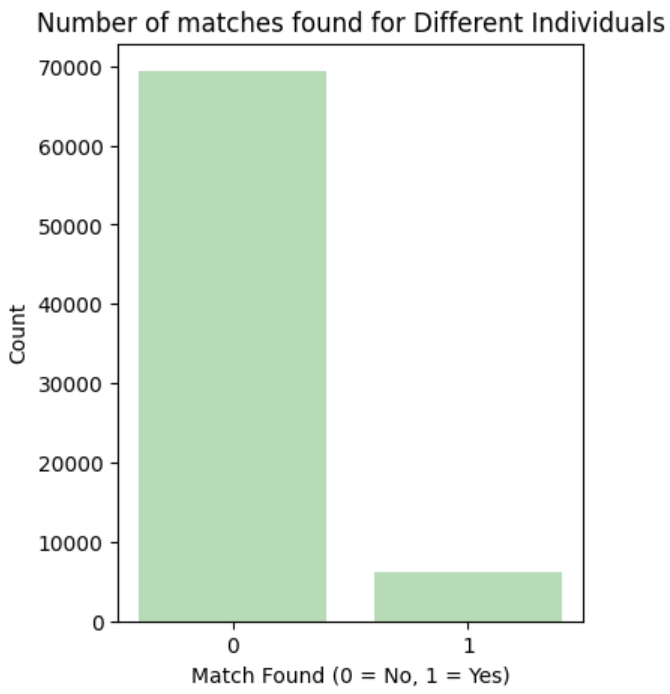
\includegraphics[width=\linewidth,height=7cm,keepaspectratio]{latex-img/mu_diff.png}
                \caption{Count of the number of matches for Different, Aligned Biometric Samples with Single Index preHashing}
                \label{mu_diff}
            \end{subfigure}
            \caption{Comparison of match counts for Same and Different Aligned Biometric Samples}
        \end{figure}
    \end{itemize}
\end{enumerate}

In our analysis of the dataset at hand featuring biometric data from 20 unique individuals, we have quantified the performance of the preHash function in distinguishing between identical and different biometric subjects. Specifically, when evaluating samples from the same individual, the probability that the preHash function will produce the same index is approximately \(22.05\%\). Conversely, when the function is applied to samples from different individuals, the probability of a match in the indices drops to roughly \(8.25\%\). This indicates that the likelihood of mistakenly identifying different individuals as the same is about three times lower than correctly matching samples from the same individual, demonstrating the preHash function's relative efficacy in biometric differentiation within this specific dataset. Moreover, we can observe that the experimental results that we got are very close to the theoretical values predicted from Table~\ref{tab:approximation_mu_taylor}. This shows that our theoretical framework and the Taylor series approximations accurately model the behavior of \(\mu_{\text{diff}}\) and \(\mu_{\text{same}}\). The minor differences between the theoretical model and the experiments can be explained by the fact that real-world biometric data can include noise and measurement errors that are not accounted for in the theoretical model.


\subsubsection{Experimental Derivation of the Probabilities \(\mu_{same}\) and \(\mu_{diff}\) Excluding the Post-Alignment Step}

We conducted an experimental investigation to determine the impact of omitting the Miura Marching step, which optimizes offsets before comparing images, on the coincidence probabilities of the indices. The Miura Matching step serves as a post-alignment phase in the current pipeline. According to Equation~\ref{eq:mu_leq}, excluding the Miura Matching phase should result in the probabilities of matching indices being less than or equal to the previous values determined for \(\mu_{\text{same}}\) and \(\mu_{\text{diff}}\), respectively.
Following the setup and conductin the experiment as described in the previous section, we obtained the following statistical analysis and probability computations:


\begin{itemize}
    \item \text{\(\mu_{\text{same}}^{obs}\)}: 
    
    \[ \mu_{\text{same}}^{obs} \approx 0.11871 = 11.87\%\]
    
    \item \text{\(\mu_{\text{diff}}^{obs}\)}:
    
    \[ \mu_{\text{diff}}^{obs} \approx 0.05651 = 5.65\% \]

    \begin{figure}[H]
        \centering
        \begin{minipage}[b]{0.48\linewidth}
            \centering
            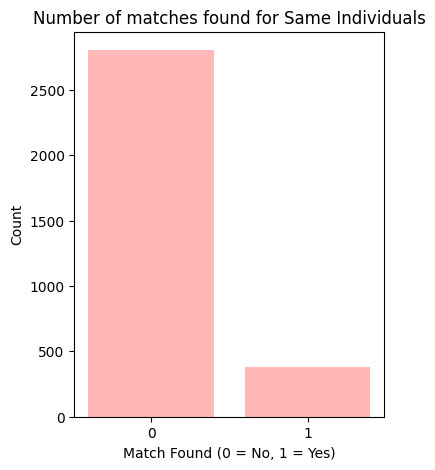
\includegraphics[width=\linewidth,height=7cm,keepaspectratio]{latex-img/mu_same_without_postAlignment.png}
            \caption{Count of the number of matches for Same, Non-Aligned Biometric Samples with Single Index preHashing}
            \label{mu_same_without_postAlignement}
        \end{minipage}
        \hfill
        \begin{minipage}[b]{0.48\linewidth}
            \centering
            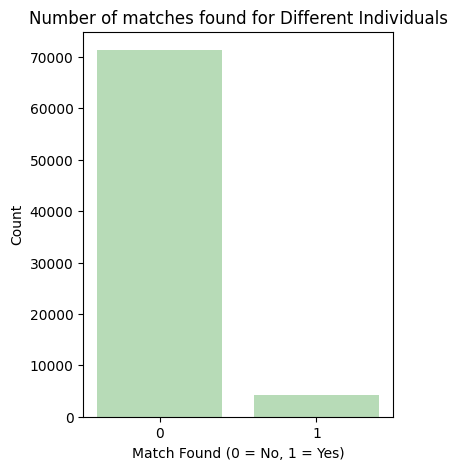
\includegraphics[width=\linewidth,height=7cm,keepaspectratio]{latex-img/mu_diff_without_postAlignment.png}
            \caption{Count of the number of matches for Different, Non-Aligned Biometric Samples with Single Index preHashing}
            \label{mu_diff_without_postAlignement}
        \end{minipage}
        \caption{Comparison of match counts for Same and Different Non-Aligned Biometric Samples}
    \end{figure}
\end{itemize}

As expected, omitting the Miura Matching step resulted in \(\mu_{\text{same}} = 11.87\%\) and \(\mu_{\text{diff}} = 5.65\%\), which are indeed less than the previously determined values of \(\mu_{\text{same}} = 22.05\%\) and \(\mu_{\text{diff}} = 8.25\%\).

